% !TeX encoding = UTF-8
% !TeX program = pdfLaTeX
% !TeX spellcheck = en_US

\documentclass[dvipsnames]{beamer}

\usepackage[T1]{fontenc}
\usepackage[utf8]{inputenc}
\usepackage[english]{babel}
\usepackage[babel]{csquotes}
\usepackage{lmodern}
\usepackage{beamerthemeshadow}
\usepackage{BeamerColor}
\usepackage{grffile}
\usepackage{microtype}
\usepackage{tabularx,booktabs,siunitx}
\usepackage[backend=biber]{biblatex}
\usepackage{tikz}
\usetikzlibrary{chains,calc,fit,shapes.geometric,decorations.pathreplacing}
\usetikzlibrary{fadings}


\frenchspacing
\graphicspath {
  {./img/},
  {./plot-wifispeeds/}, {./plot-jump-stats/},  {./plot-measurements/},
  {./plot-mode-calculation/}, {./plot-measurements-delta-delta/},
  {./plot-execution/}
}
\addbibresource{references.bib}
\defbibheading{references}[]{\section*{#1}}
\setbeamertemplate{bibliography item}{%
  \ifboolexpr{ test {\ifentrytype{book}} or test {\ifentrytype{mvbook}}
    or test {\ifentrytype{collection}} or test {\ifentrytype{mvcollection}}
    or test {\ifentrytype{reference}} or test {\ifentrytype{mvreference}} }
    {\setbeamertemplate{bibliography item}[book]}
    {\ifentrytype{online}
       {\setbeamertemplate{bibliography item}[online]}
       {\setbeamertemplate{bibliography item}[article]}}%
  \usebeamertemplate{bibliography item}}
\defbibenvironment{bibliography}
  {\list{}
     {\settowidth{\labelwidth}{\usebeamertemplate{bibliography item}}%
      \setlength{\leftmargin}{\labelwidth}%
      \setlength{\labelsep}{\biblabelsep}%
      \addtolength{\leftmargin}{\labelsep}%
      \setlength{\itemsep}{\bibitemsep}%
      \setlength{\parsep}{\bibparsep}}}
  {\endlist}
  {\item}
\newcommand\FrameRIMOSSO[1]{}
\makeatletter
\newcommand{\rulecolor}[1]{%
  \def\CT@arc@{\color{#1}}%
}
\newcommand*\unit{\,\mathrm}
\newcommand<>\xcancelthistikz[1][]{%
  \only#2{
    \draw [#1] ($(current bounding box.north west)+(1pt,-1pt)$) --
     ($(current bounding box.south east)+(-1pt,1pt)$);
    \draw [#1] ($(current bounding box.north east)+(-1pt,-1pt)$) --
     ($(current bounding box.south west)+(1pt,1pt)$);
  }
}
\let\oldinsertshorttitle\insertshorttitle
\newcommand*\newinsertshorttitle{%
  \oldinsertshorttitle\hfill%
  \insertframenumber\,/\,\inserttotalframenumber}
\newcommand*\noframenumber{%
  \addtocounter{framenumber}{-1}%
  \let\insertshorttitle\oldinsertshorttitle
}
\let\insertshorttitle\newinsertshorttitle
\makeatother


\title[An implementation of \textsl{pathrate} on Android]{%
  \textsl{Pathrate} on mobile environments\texorpdfstring{\\}{--}
  An implementation on Android
}
\author{
  Antonio Macrì\texorpdfstring{ $\cdot$}{,}
  Francesco Racciatti\texorpdfstring{ $\cdot$}{,}
  Silvia Volpe
}
\renewcommand*\year{2013}
\renewcommand*\month{7}
\renewcommand*\day{8}
\date{\today}


\begin{document}

\frame{\noframenumber
  \titlepage
}

\frame{\frametitle{\contentsname}\noframenumber
  \tableofcontents
}


\section{How \protect\textsl{pathrate} works}
\frame{\sectionpage\noframenumber}


\frame{\frametitle{Pathrate}
 \begin{block}{Pathrate goal}
   Pathrate is a tool that calculates the capacity of a path.
  \end{block}

 \bigskip
 It works in 2 steps:
 \begin{description}
 \item[phase 1] uses packet pairs to obtain a set of capacity estimations
 \item[phase 2] uses packet trains to compute the lower bound of the capacity
 \end{description}
}


\subsection{Packet-pair technique}

\frame{\frametitle{Packet-pair technique}
  %Pathrate estimates the capacity of a path using the \emph{packet-pair
  %technique}

  \begin{block}{Scenario}
  Two consecutive \emph{probing packets} leave the sender \emph{back-to-back}
  and arrive at the receiver with a \emph{dispersion} (spacing) that is
  determined by the \emph{narrow link} in the path
  \end{block}

  \bigskip
  \bigskip
  \begin{columns}
  \begin{column}{0.7\columnwidth}\scriptsize
  \begin{tikzpicture}[fill=LightBlue, node distance=0.1em]
    \begin{scope}[start chain=1 going right, minimum width=1em, minimum height=3.5em]
      \node [draw, fill, on chain=1] (a) {};
      \node [draw, fill, on chain=1] {};
      \node [draw, fill, on chain=1] {};
      \node [draw, fill, on chain=1] (d) {};
    \end{scope}
    \node [draw, fill, trapezium, right=of d, minimum width=3.5em,
      rotate=-90, anchor=south, trapezium angle=40] (e) {};
    \begin{scope}[start chain=1 going right, minimum width=3.5em, minimum height=1em]
      \node [draw, fill, on chain=1, right=of e.north] (f) {};
      \node [draw, fill, on chain=1, right=of f] (g) {};
      \node [draw, fill, on chain=1, right=of g] (h) {};
    \end{scope}
    \node [draw, fill, trapezium, right=of h, minimum width=3.5em,
      rotate=90, anchor=north, trapezium angle=40] (i) {};
    \begin{scope}[start chain=1 going right, minimum width=1em, minimum height=3.5em]
      \node [draw, fill, on chain=1, right=2.4em of i.south] (j) {};
      \node [draw, fill, on chain=1, right=2.4em of j] (k) {};
    \end{scope}
    \draw[|-|] ($(g.south west)+(0,-1em)$) -- node[below] {$\delta$}
      ($(h.south west)+(0,-1em)$);
    \draw[|-|] ($(j.south west)+(0,-1em)$) -- node[below] {$\delta$}
      ($(k.south west)+(0,-1em)$);
    \draw[black, thick, dotted, -stealth] (k.east) -- ++(1.3em,0);
    \draw[black, thick, dotted, stealth-] (a.west) -- ++(-1em,0);
    \coordinate (sendertopleft) at ($(a.north west)+(-1.5em,0.2em)$);
    \coordinate (sendertopright) at ($(e.bottom left corner)+(0.1em,0.2em)$);
    \coordinate (senderbottomleft) at ($(a.south west)+(-1.5em,-0.2em)$);
    \coordinate (senderbottomright) at ($(e.bottom right corner)+(0.1em,-0.2em)$);
    \coordinate (pipetopleft) at ($(f.north west)+(-0,0.2em)$);
    \coordinate (pipetopright) at ($(h.north east)+(0,0.2em)$);
    \coordinate (pipebottomleft) at ($(f.south west)+(-0,-0.2em)$);
    \coordinate (pipebottomright) at ($(h.south east)+(0,-0.2em)$);
    \coordinate (receivertopleft) at ($(i.bottom right corner)+(-0.1em,0.2em)$);
    \coordinate (receivertopright) at ($(k.north east)+(1.5em,0.2em)$);
    \coordinate (receiverbottomleft) at ($(i.bottom left corner)+(-0.1em,-0.2em)$);
    \coordinate (receiverbottomright) at ($(k.south east)+(1.5em,-0.2em)$);
    \draw[rounded corners=5pt] (sendertopleft) -- (sendertopright) --
      (pipetopleft) -- (pipetopright) -- (receivertopleft) -- (receivertopright);
    \draw[rounded corners=5pt] (senderbottomleft) -- (senderbottomright) --
      (pipebottomleft) -- (pipebottomright) -- (receiverbottomleft) --
      (receiverbottomright);
  \end{tikzpicture}
  \end{column}\hfill
  \begin{column}{0.17\columnwidth}
  $b = L/\delta$
  \end{column}
  \end{columns}
}


\subsection{Capacity modes}

\frame{\frametitle{Capacity modes}
  \begin{block}{Packet-pair bandwidth distribution}
    All capacities are used to compute a probability density function called the
    \emph{packet-pair bandwidth distribution} $\mathcal{B}$
  \end{block}

  \begin{center}
  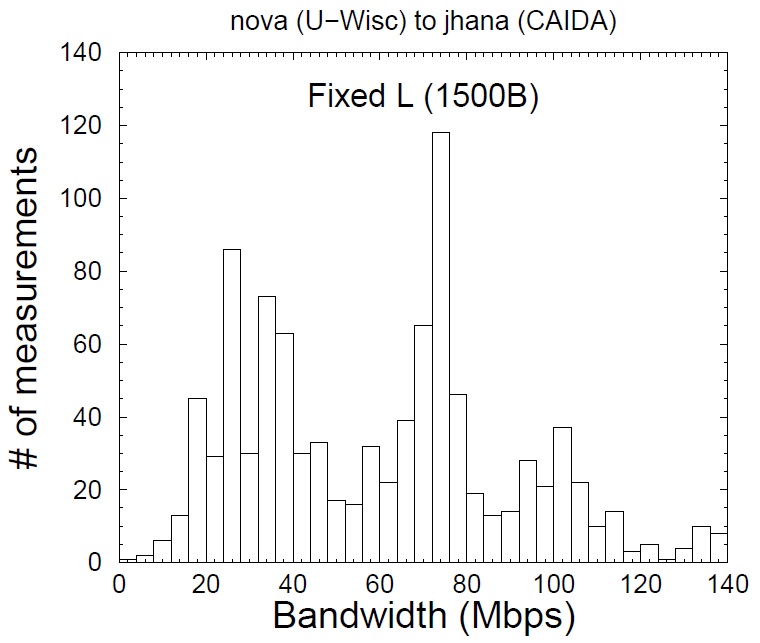
\includegraphics[width=0.45\textwidth]{example-multimodal}
  \end{center}
}

\frame{\frametitle{Capacity modes (cont.)}
  \begin{alertblock}{Problem 1}
  The distribution of the capacities is \emph{multimodal}
  \end{alertblock}

  \begin{columns}[T]
  \begin{column}{0.45\columnwidth}
  \begin{alertblock}{Problem 2}
    The correct path capacity is likely to be the global mode only when the path
    is \emph{lightly loaded}
  \end{alertblock}
  \end{column}
  \begin{column}{0.45\textwidth}
  \resizebox{!}{0.95\columnwidth}{\begin{tikzpicture}[font=\fontsize{5}{0}\selectfont]
    \node (img) {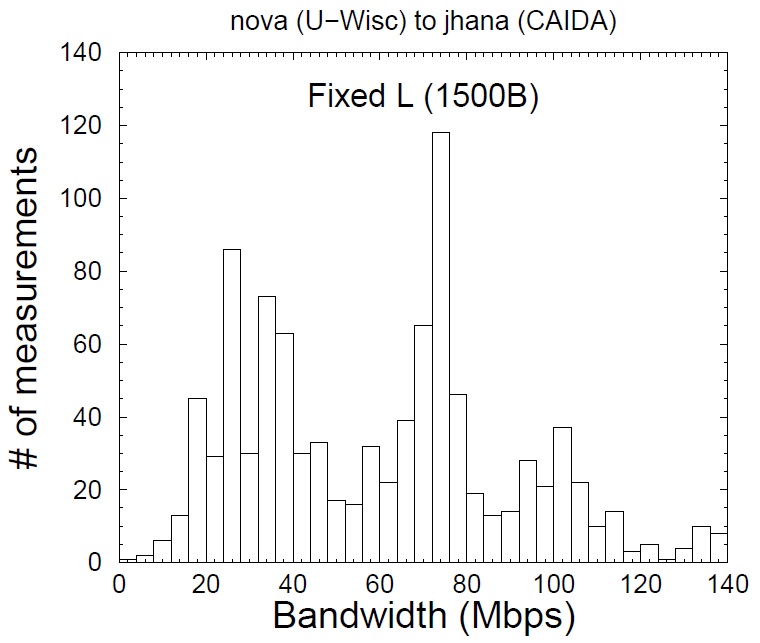
\includegraphics[width=0.7\textwidth]{example-multimodal}};
    \coordinate (cm) at ($(img.north west)!0.734!(img.south east)+(0,1em)$);
    \node<2>[red, above] at ($(cm)+(0.2em,1.2em)$) (label) {Path capacity};
    \draw<2>[red, -stealth] (label) -- (cm);
  \end{tikzpicture}}
  \end{column}
  \end{columns}
}

\frame{\frametitle{Capacity modes (cont.)}
  \begin{center}
  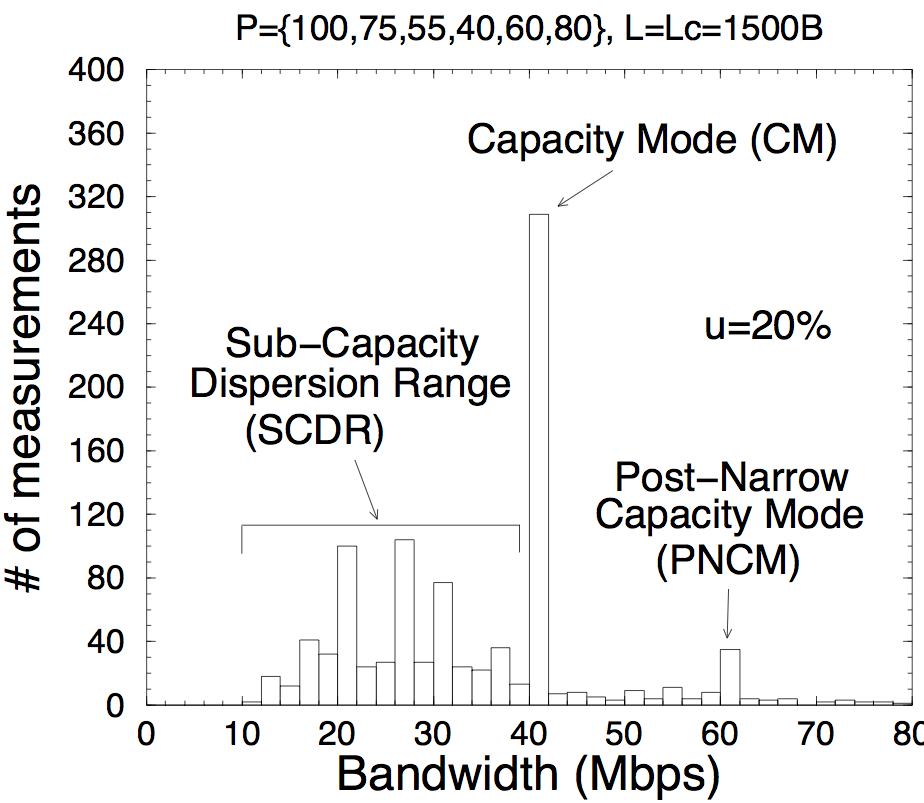
\includegraphics[width=0.48\columnwidth]{capacity-modes-u20}\quad
  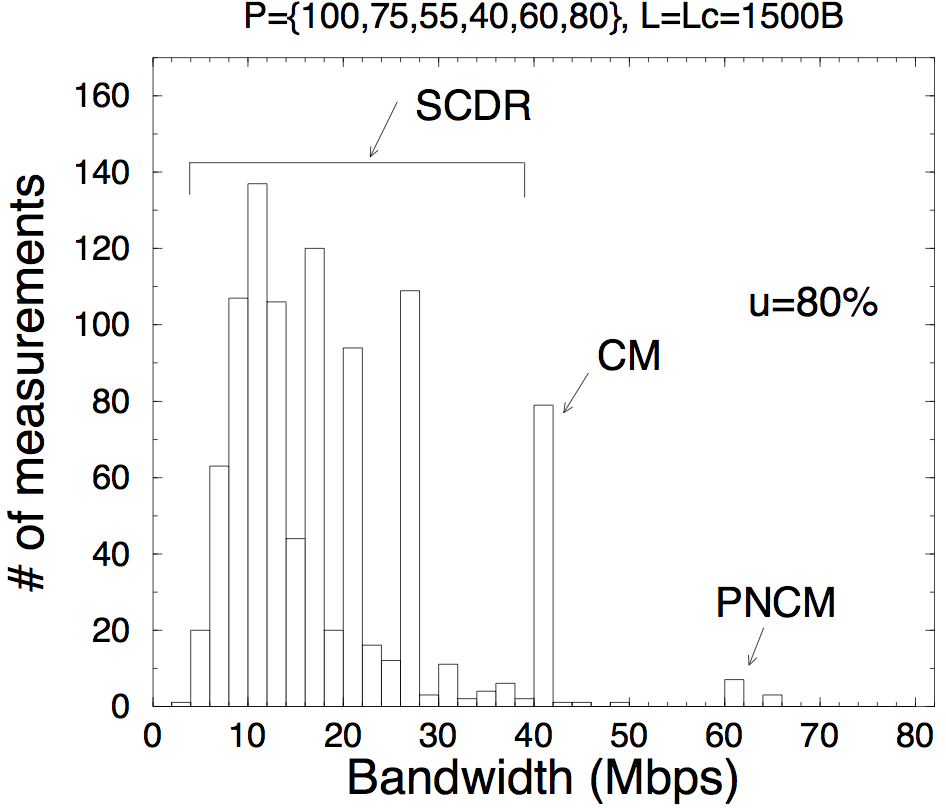
\includegraphics[width=0.48\columnwidth]{capacity-modes-u80}
  \end{center}
}

\frame{\frametitle{Capacity modes (cont.)}
  \begin{block}{Wrong estimations}
  Underestimations due to cross-traffic (SCDR zone)
  \end{block}
  \vfill

  \begin{center}\footnotesize
  \begin{tikzpicture}[fill=LightBlue, node distance=0.3em]
    \newcommand*\lt{0.5em}\newcommand*\mltp{3}
    \begin{scope}[start chain=1 going left, minimum width=5em]
      \node [draw, fill, on chain=1] (first-p1) {Probe 1};
      \node [draw, fill=red!50, on chain=1] (first-interf) {Interf.};
      \node [draw, fill, on chain=1] (first-p2) {Probe 2};
      \draw [|-|, red] ($(first-p1.south west)+(0,-\lt)$) -- ($(first-p2.south west)+(0,-\lt)$);
    \end{scope}
    \begin{scope}[start chain=1 going left, minimum width=5em]
      \node [draw, fill, on chain=1, below=\mltp*\lt of first-p1] (second-p1) {Probe 1};
      \node [draw, fill=red!50, on chain=1, minimum width=4em] {Interf.};
      \node [draw, fill, on chain=1] (second-p2) {Probe 2};
      \draw [|-|, red] ($(second-p1.south west)+(0,-\lt)$) --
        ($(second-p2.south west)+(0,-\lt)$);
    \end{scope}
    \begin{scope}[start chain=1 going left, minimum width=5em]
      \node [draw, fill, on chain=1, below=\mltp*\lt of second-p1] (third-p1) {Probe 1};
      \node [draw, fill=red!50, on chain=1, minimum width=8em] {Interf.};
      \node [draw, fill, on chain=1] (third-p2) {Probe 2};
      \draw [|-|, red] ($(third-p1.south west)+(0,-\lt)$) -- ($(third-p2.south west)+(0,-\lt)$);
    \end{scope}
    \draw[|-|] ($(first-interf.north west)+(0,\mltp*\lt)$) -- node[above] {Ideal dispersion}
      ($(first-p1.north west)+(0,\mltp*\lt)$);
    \coordinate (receiver-top-left) at ($(first-p1.north east)+(2em,0)$);
    \coordinate (receiver-bottom-right) at ($(third-p1.south east)+(4em,0)$);
    \node [fit=(receiver-top-left)(receiver-bottom-right), draw,
      label={center:\rotatebox{90}{Receiver}}] (receiver) {};
    \begin{scope}[black, thick, dotted, -stealth]
      \draw (first-p1) -- (receiver.west |- first-p1);
      \draw (second-p1) -- (receiver.west |- second-p1);
      \draw (third-p1) -- (receiver.west |- third-p1);
    \end{scope}
  \end{tikzpicture}
  \end{center}
}

\frame{\frametitle{Capacity modes (cont.)}
  \begin{block}{Wrong estimations}
  Overestimations due to non-empty buffers in some post-narrow node (PNCMs)
  \end{block}
  \vfill

  \begin{center}\footnotesize
  \begin{tikzpicture}[fill=LightBlue, node distance=0.1em]
    \begin{scope}[start chain=1 going left, minimum width=1em, minimum height=5em]
      \node [draw, fill, on chain=1] (head) {};
      \node [draw, fill, on chain=1] {};
      \node [draw, fill, on chain=1] {};
      \node [draw, fill, on chain=1] (tail) {};
    \end{scope}
    \begin{scope}[start chain=1 going left, minimum width=5em]
      \node [draw, fill, on chain=1, left=5em of tail] (probe-1) {Probe 1};
      \node [draw, fill, on chain=1, left=4em of probe-1] (probe-2) {Probe 2};
    \end{scope}
    \draw[black, thick, dotted, -stealth] (head.east) -- ++(1em,0);
    \coordinate (pipetopleft) at ($(probe-2.north west)+(-1.5em,0.2em)$);
    \coordinate (pipetopright) at ($(probe-1.north east)+(0.5em,0.2em)$);
    \coordinate (pipebottomleft) at ($(probe-2.south west)+(-1.5em,-0.2em)$);
    \coordinate (pipebottomright) at ($(probe-1.south east)+(0.5em,-0.2em)$);
    \coordinate (topleft) at ($(tail.north west)+(-2.5em,0.2em)$);
    \coordinate (topright) at ($(head.north east)+(0.5em,0.2em)$);
    \coordinate (bottomleft) at ($(tail.south west)+(-2.5em,-0.2em)$);
    \coordinate (bottomright) at ($(head.south east)+(0.5em,-0.2em)$);
    \draw[rounded corners=5pt] (pipetopleft) -- (pipetopright) -- (topleft) -- (topright);
    \draw[rounded corners=5pt] (pipebottomleft) -- (pipebottomright) --
      (bottomleft) -- node[below] {Buffer} (bottomright);
  \end{tikzpicture}
  \end{center}
}


\subsection{Packet trains}

\frame{\frametitle{Packet trains}
  Generalization: using packet trains ($N>2$ back-to-back packets of the same
  size $L$) we can calculate the bandwith as:
  \[b(N) = \frac{(N-1)L}{\Delta(N)}\]
  \pause

  When the train length $N$ is sufficiently large, bandwidth measurements tend
  toward a single value leading to a unimodal distribution that becomes
  \emph{independent of~$N$}: this value is called the \emph{Average Dispersion
  Rate} (ADR)
}

\frame{\frametitle{Average Dispersion Rate}
 \begin{center}
  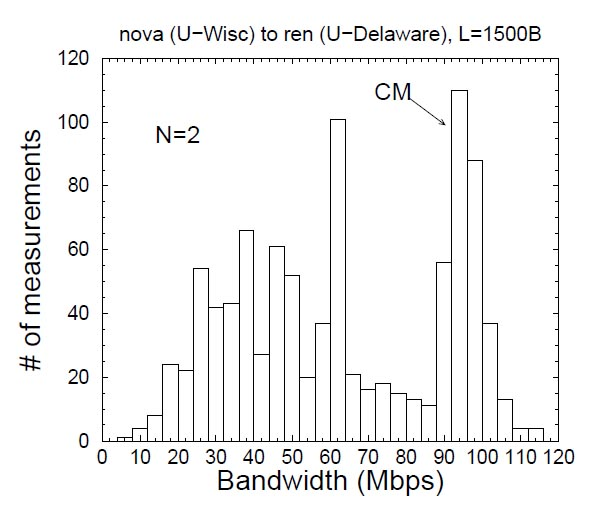
\includegraphics[width=0.48\columnwidth]{trainLength2}\quad
  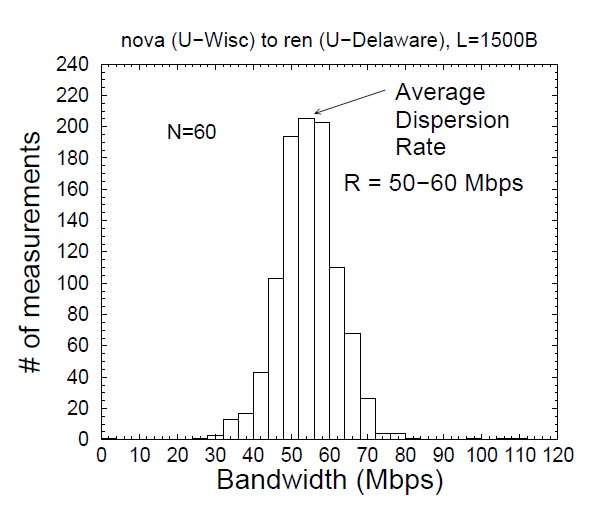
\includegraphics[width=0.48\columnwidth]{trainLength60}
  \end{center}
}


\subsection{Capacity estimation methodology}

\frame{\frametitle{Capacity estimation methodology}
  \begin{exampleblock}{SCDR and PNCMs countermeasures}
    Varying probing packet size among different packet pairs makes SCDR modes
    wider and weaker. Probing packets as large as possible (but not too much)
    reduce the creation of PNCMs
  \end{exampleblock}
  \pause

  \begin{exampleblock}{ADR as lower bound}
    The ADR is a \emph{lower bound} of the capacity
    % and an \emph{upper bound} of the available bandwidth 
    of the path
  \end{exampleblock}
  \pause

  \begin{exampleblock}{Final capacity estimate}
    In the packet pair bandwidth distribution, ignore modes below the ADR mode
    and choose the one with the maximum \emph{figure of merit}
  \end{exampleblock}
}



\section{\protect\textsl{pathrate} in mobile environments}
\frame{\sectionpage\noframenumber}


\subsection{Main problems}

\frame{\frametitle{Main problems}
  Why do not port \textsl{pathrate} to Android?
  \begin{itemize}
  \item long running time ($15\div30$ mins)
  \pause
  \item no care for consumed traffic ($100\div180$\,MB)
  \pause
%  \item not tuned for wireless communications
%  \pause
  \item not suitable for energy-constrained devices
  \end{itemize}
}

%slide commentata per volere di silvia
\iffalse
\frame{\frametitle{Not tuned for wireless communications}
  \begin{itemize}
  \item Contention for the shared medium
  \item Possible high BER
  \end{itemize}

  \vspace{-4\baselineskip}
  \begin{flushright}
  \begin{tikzpicture}[node distance=0.4em and -1.6em]
  \node (wireless-router) {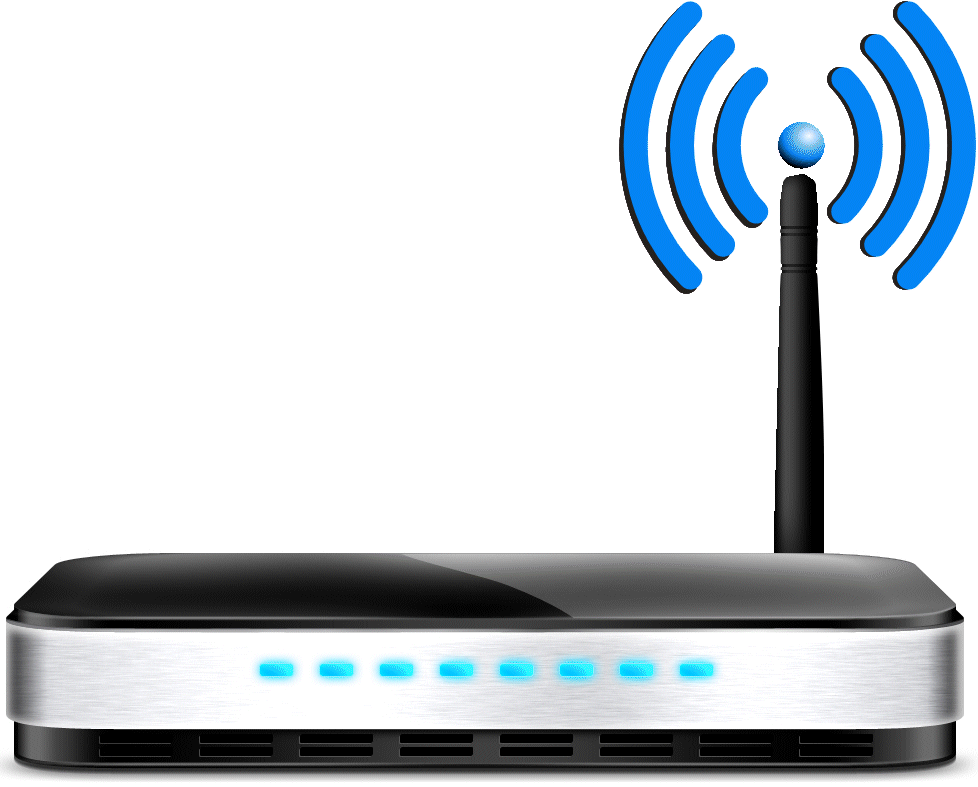
\includegraphics[width=4em]{router}};
  \node [below left=of wireless-router] (left-waves)
    {\reflectbox{
\includegraphics[width=2em]{waves}}};
  \node [below right=of wireless-router] (right-waves) {
\includegraphics[width=2em]{waves}};
  \node [below left=of left-waves] {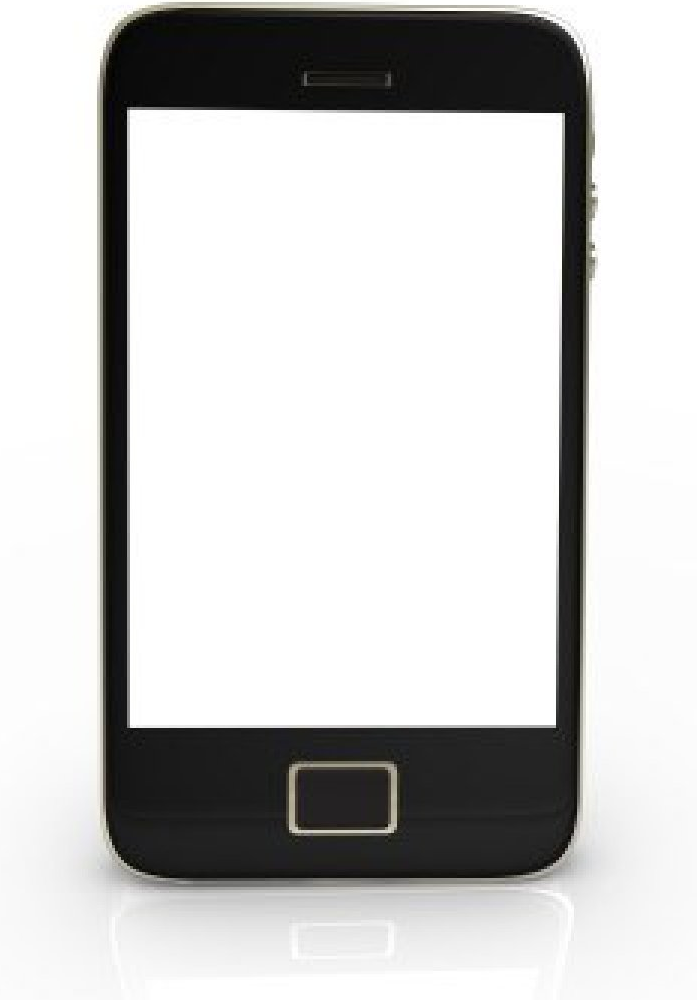
\includegraphics[width=2em]{smartphone2}};
  \node [below right=of right-waves] {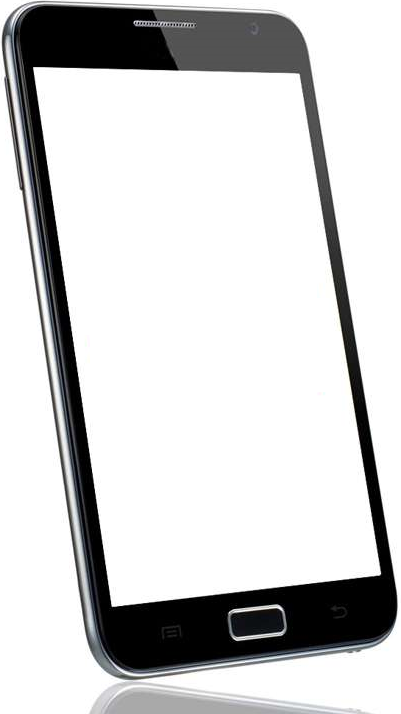
\includegraphics[width=1.6em]{smartphone}};
  \end{tikzpicture}
  \end{flushright}
}
\fi


\frame{\frametitle{Not suitable for energy-constrained devices}
  \begin{itemize}
  \item<+-> CPU frequency is scaled based on battery level or current load
  \item<+-> NIC rate depends on channel conditions
  \begin{center}\visible<.->{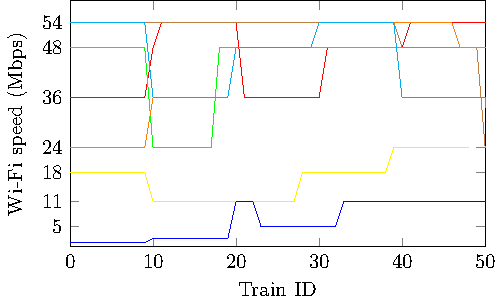
\includegraphics[width=0.7\textwidth]{wifispeeds}}
  \end{center}
  \setbeamercolor{item}{fg=red}
  \item<+-> Network device driver may activate \emph{Interrupt Coalescence} (IC)
  \end{itemize}
}


\subsection{Interrupt Coalescence}

\frame{\frametitle{Interrupt Coalescence}
  \begin{center}
  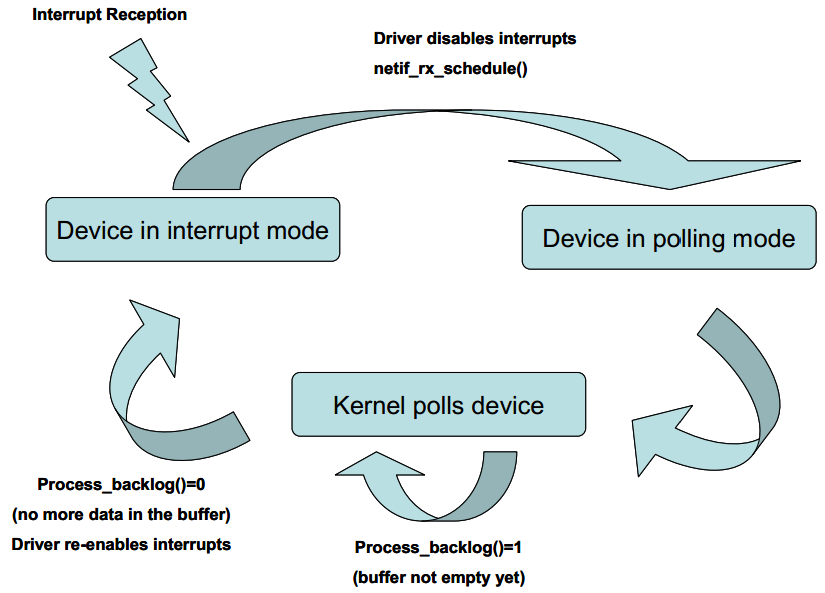
\includegraphics[width=0.75\textwidth]{napi-intel}
  \end{center}
}

\frame{\frametitle{Interrupt Coalescence in wired environment}
  \begin{columns}[c]
  \begin{column}{0.45\columnwidth}
  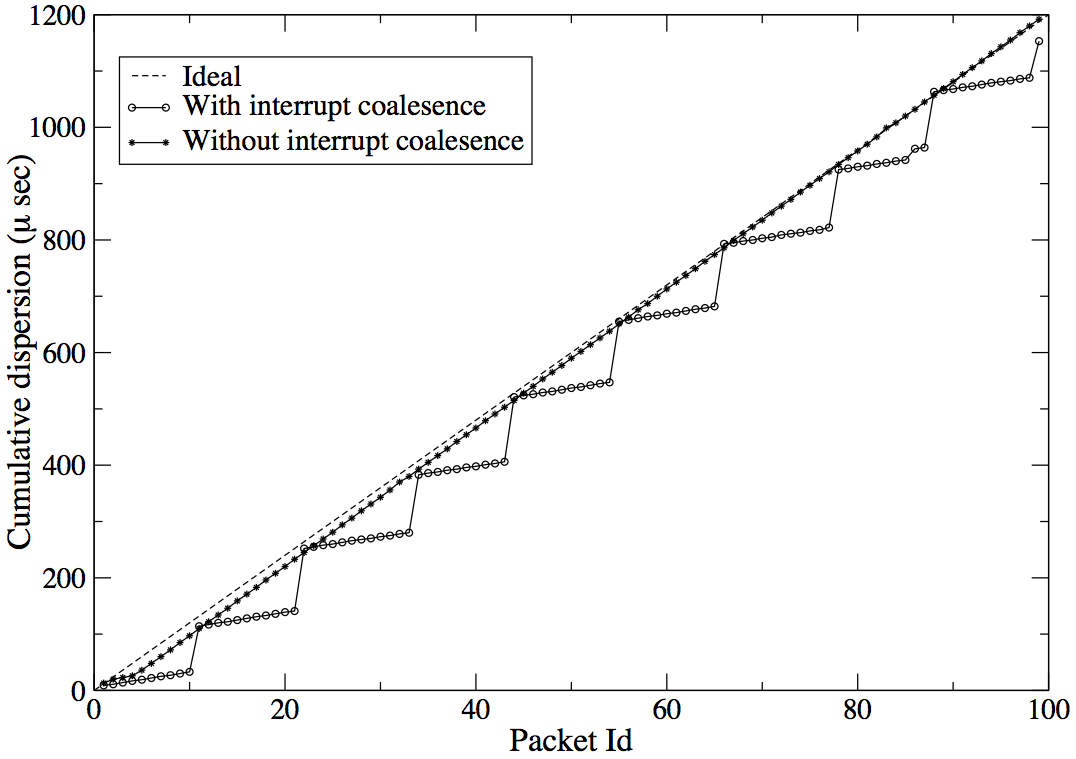
\includegraphics[width=\columnwidth]{interrupt-coalescence-wired}
  \end{column}
  \pause
  \begin{column}{0.46\columnwidth}
  \begin{exampleblock}{Detect IC}
    \textsl{pathrate} detects coalescence by sending a back-to-back packet
    train and comparing (at the receiver) measured dispersions with the
    kernel-to-user latency $\delta_\textup{k-u}$
  \end{exampleblock}
  \end{column}
  \end{columns}
  \medskip
  \pause
  \begin{exampleblock}{Capacity from IC}
    In case of IC, the capacity of the path can be calculated by dividing the
    plateau length by the jump height
  \end{exampleblock}
}

\frame{\frametitle{Interrupt Coalescence in mobile environment}
  \begin{alertblock}{Problems}
  \begin{itemize}
   \item In the NIC buffer there are packets for other applications
   \pause
   \item Kernel can adapt CPU frequency to computational load and battery level
   \pause
   \item Timer resolution can be insufficient ($30\unit{\mu s}$)
   \pause
%   \item decrease timer resolution means visibly increase battery consumption 
   \item Height of jump depends on many factors, not only packet buffering
         (e.\,g. context switches, scheduling mechanisms)
   \end{itemize}
  \end{alertblock}
  \pause

  \begin{block}{Pseudo-IC}
   Due to these factors the observed behavior is highly variable. Then, in mobile environment
   it is more correct to talk about pseudo-IC rather than simple IC.
  \end{block}
}


\subsection{IC distortions}

\frame{\frametitle{Pseudo-IC}
  \begin{center}
  \begin{tikzpicture}[node distance = 9em]
  \node (A) {\includegraphics[width=0.3\textwidth,page=4]{Receiver-2013.06.12-6}};
  \node [right of = A, xshift=2em] (B)
    {\includegraphics[width=0.3\textwidth, page=2]{Receiver-2013.06.12-6}};
  \node [below of = A, xshift=5.5em] (C)
    {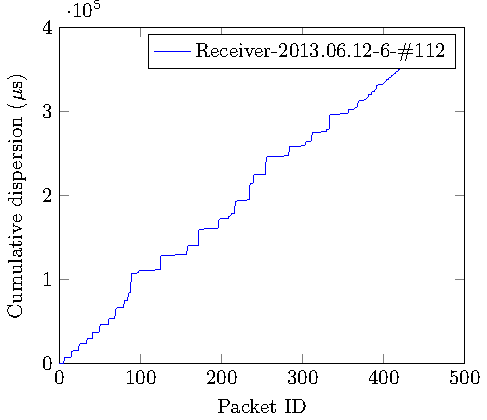
\includegraphics[width=0.3\textwidth,page=1]{Receiver-2013.06.12-6}};
  \node [red, xshift = -1.7em, yshift = 1.5em] at (A) (A1)
    {\Tiny{running with interrupt}};
  \draw [red, -stealth] (A1.south) -- ++(0, -3em);

  \visible<2->{
    \node [red, xshift = 2em, yshift= 1em ] at (A) (A2)
      {\Tiny running with pseudo-IC};
    \draw [red, -stealth] (A2.south) -- ++ (-1em,-1.8em);
    \draw [red, -stealth] (A2.south) -- ++ (1em,-1.2em);
  }
  \visible<3->{
    \node [red, xshift = 2.5em, yshift = -2.5em ] at (B) (B2)
      {\Tiny running with interrupt};
    \draw [red, -stealth] (B2.west) -- ++ (-3em, 0em);
    \draw [red, -stealth] (B2.north) -- ++ (0, 3.5em);
  }
  \visible<4->{
    \node [red, xshift = -1.5em, yshift = 2em ] at (B) (B1)
      {\Tiny running with pseudo-IC};
    \draw [red, -stealth] (B1.south) -- ++ (.8em, -1.2em);
  }
  \visible<5->{
    \node [red, xshift = 1em, yshift = -1.7em ] at (C) (C1)
      {\Tiny running with only pseudo-IC};
  }
  \end{tikzpicture}
  \end{center}
}

\frame{\frametitle{Pseudo-IC (cont.)}
  \begin{columns}[c]
  \begin{column}{0.45\columnwidth}
  \newcommand*\jumpstatsfile{Clear-802.11g-WPA2-2}
  \includegraphics[width=0.9\textwidth, page=1]{\jumpstatsfile}\\
  \includegraphics[width=0.9\textwidth, page=3]{\jumpstatsfile}
  \end{column}

  \begin{column}{0.55\columnwidth}
  \begin{block}{Plateaus length \& jumps height }
  If the behavior of pseudo-IC was regular then all the occurrences would
  be concentrated around a single value.
  The same speech applies to jumps height.
  \end{block}
  \end{column}
  \end{columns}

\iffalse
  \begin{center}
  \newcommand*\jumpstatsfile{Clear-802.11g-WPA2-2}
  \includegraphics[width=0.34\textwidth, page=1]{\jumpstatsfile}\\
  \includegraphics[width=0.34\textwidth, page=3]{\jumpstatsfile}
  \end{center}
  \fi
}

\frame{\frametitle{Pseudo-IC (cont.)}
   \begin{exampleblock}{Calculation of path capacity}
   Pseudo-IC patterns are very irregular then it is not possible to calculate
   capacity with jumps and plateaus.
  \end{exampleblock}

  \begin{center}
  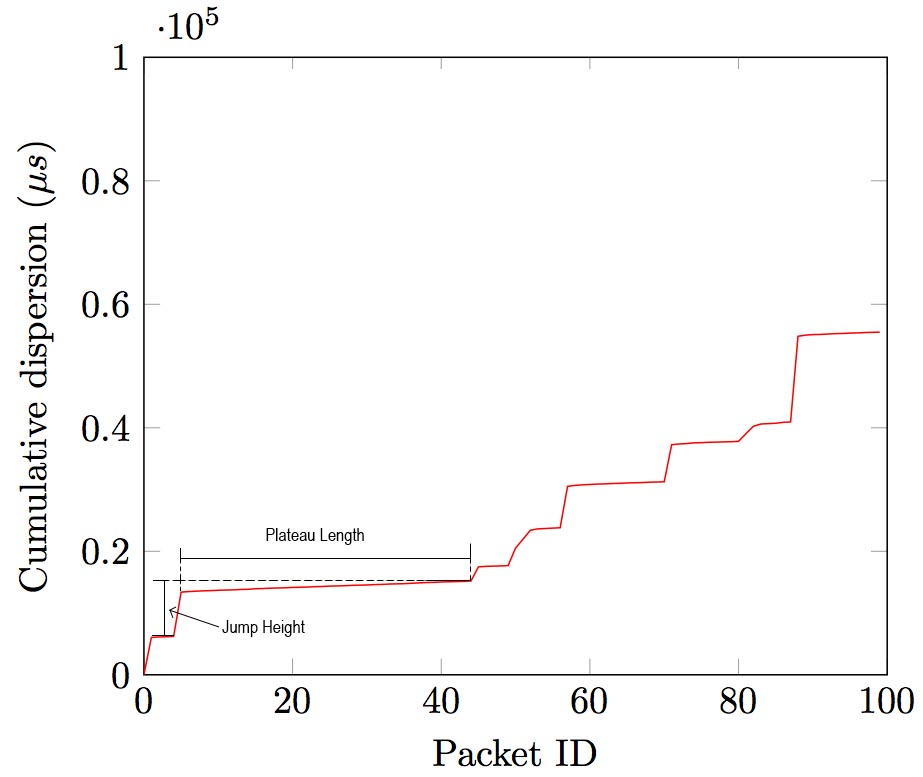
\includegraphics[width=0.5\textwidth]{capacity-plateau2}
  \end{center}
  \smallskip
 }



\section{SmartPathrate}
\frame{\sectionpage\noframenumber}


\subsection{Objectives}

\frame{\frametitle{Our objectives}
  The execution of our application
  \begin{itemize}
  \item should not take a long time
    \begin{itemize}
    \item user wants to have a result quickly
    \item battery life should not be significantly affected
    \end{itemize}
    \pause
  \item should not require too much resources
    \begin{itemize}
    \item processing complexity of mathematical computations
    \item memory usage for buffering partial results
    \end{itemize}
    \pause
  \item should use as less data as possible
    \begin{itemize}
    \item mobile data plan may have traffic limitations
    \item more data means more processing
    \end{itemize}
  \end{itemize}
}


\subsection{Efficiency}

\frame{\frametitle{Packet pairs vs packet trains}
  \begin{itemize}
  \item Pathrate: spacing between consecutive pairs
  \begin{itemize}
  \item to avoid late packets interfere with subsequent pairs
  \item drop pair in case of interference or packet losses
  \end{itemize}
  \begin{center}\tiny
  \begin{tikzpicture}[fill=LightBlue, node distance=0.1em]
    \newcommand*\pcount{3} \newcommand*\lastx{}
    \coordinate (p-2);
    \begin{scope}[start chain=1 going left, minimum width=4em]
      \foreach \x [remember=\x as \lastx] in {1,...,\pcount} {
        \node [draw, fill, on chain=1, left=6em of p\lastx-2] (p\x-1) {Probe 1};
        \node [draw, fill, on chain=1] (p\x-2) {Probe 2};
        \ifx\lastx\empty\else
          \draw[decorate, decoration={brace,amplitude=0.5em}, black!90]
            ($(p\lastx-2.south west)-(0,0.5em)$) -- ($(p\x-1.south east)-(0,0.5em)$)
            node[midway,anchor=north,yshift=-1.5ex] {Wait};
        \fi
      }
    \end{scope}
    \draw[-stealth, dashed, black] ($(p1-1.east)+(0.5em,0)$) -- ++(3em,0);
    \coordinate (pipetopleft) at ($(p\pcount-2.north west)+(-1.5em,0.2em)$);
    \coordinate (pipetopright) at ($(p1-1.north east)+(0.5em,0.2em)$);
    \coordinate (pipebottomleft) at ($(p\pcount-2.south west)+(-1.5em,-0.2em)$);
    \coordinate (pipebottomright) at ($(p1-1.south east)+(0.5em,-0.2em)$);
    \draw (pipetopleft) -- (pipetopright) -- ++(3.5em,0);
    \draw (pipebottomleft) -- (pipebottomright) -- ++(3.5em,0);
  \end{tikzpicture}
  \end{center}
  \pause
  \vspace{-2ex}
  \begin{itemize}
  \item total time in wait state is at least about $12\div13$ minutes
  \end{itemize}
  \pause

  \medskip
  \item SmartPathrate: smaller spacing between trains
  \begin{itemize}
  \item treat packets from previous trains as cross traffic
  \item drop only in case of packet losses
  \end{itemize}
  \begin{center}\tiny
  \begin{tikzpicture}[fill=LightBlue, node distance=0.1em]
    \newcommand*\pcount{4} \newcommand*\lastx{1}
    \begin{scope}[start chain=1 going left, minimum width=4em]
      \node [draw, fill, on chain=1] (a1) {Probe 1};
      \foreach \x in {2,...,\pcount} {
        \node [draw, fill, on chain=1] (a\x) {Probe \x};
      }
      \node [draw, fill, on chain=1, left=3em of a\pcount] (b1) {Probe 1};
      \foreach \x in {2,...,\pcount} {
        \node [draw, fill, on chain=1] (b\x) {Probe \x};
      }
    \end{scope}
    \draw[-stealth, dashed, black] ($(a1.east)+(0.5em,0)$) -- ++(3em,0);
    \coordinate (pipetopleft) at ($(b\pcount.north west)+(-1.5em,0.2em)$);
    \coordinate (pipetopright) at ($(a1.north east)+(0.5em,0.2em)$);
    \coordinate (pipebottomleft) at ($(b\pcount.south west)+(-1.5em,-0.2em)$);
    \coordinate (pipebottomright) at ($(a1.south east)+(0.5em,-0.2em)$);
    \draw (pipetopleft) -- (pipetopright) -- ++(3.5em,0);
    \draw (pipebottomleft) -- (pipebottomright) -- ++(3.5em,0);
  \end{tikzpicture}
  \end{center}
  \end{itemize}
}

\frame{\frametitle{Processing complexity and memory usage}
  \begin{minipage}{0.95\columnwidth}
  \begin{minipage}{0.54\columnwidth}
  \vspace{1em}
  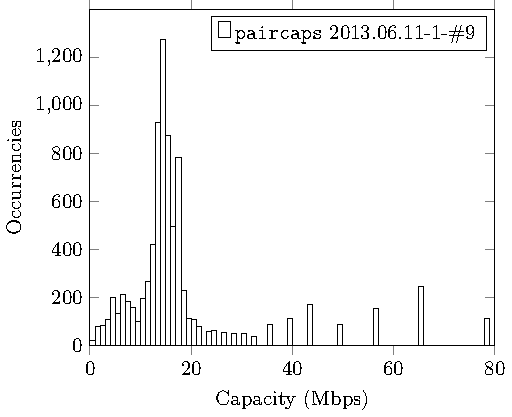
\includegraphics[width=\columnwidth]{plot-mode-calculation}
  \end{minipage}
  \hfill
  \begin{minipage}{0.38\columnwidth}
  \begin{exampleblock}{Mode calculation}\centering
    $3\cdot O(n\omega)$\\ $\Downarrow$\\ $O(n\omega) + 2\cdot O(n\log\omega)$
  \end{exampleblock}
  \begin{exampleblock}{Main change}\centering
    Linear search\\ $\Downarrow$\\ Binary search
  \end{exampleblock}
  \end{minipage}
  \end{minipage}
}

\frame{\frametitle{Data complexity}
  \begin{block}{Number of capacity estimates}
  \smallskip
  \begin{tabular}{l}
  \tiny
  \begin{tikzpicture}[fill=LightBlue, node distance=0.1em]
    \newcommand*\pcount{2} \newcommand*\lt{1em} \newcommand*\lastx{}
    \coordinate (b);
    \begin{scope}[start chain=1 going left, minimum width=4em]
      \foreach \x [remember=\x as \lastx] in {0,1,...,\pcount} {
        \node [draw, fill, on chain=1, left=3em of b\lastx] (a\x) {Probe 1};
        \node [draw, fill, on chain=1] (b\x) {Probe 2};
        \draw [|-|] ($(a\x.north west)+(0,\lt)$) -- ($(b\x.north west)+(0,\lt)$);
      }
    \end{scope}
    \draw[-stealth, dashed, black] ($(a0.east)+(0.5em,0)$) -- ++(3em,0)
      node[xshift=5em]{\normalsize$N/2$};
    \coordinate (pipetopleft) at ($(b\pcount.north west)+(-1.5em,0.2em)$);
    \coordinate (pipetopright) at ($(a0.north east)+(0.5em,0.2em)$);
    \coordinate (pipebottomleft) at ($(b\pcount.south west)+(-1.5em,-0.2em)$);
    \coordinate (pipebottomright) at ($(a0.south east)+(0.5em,-0.2em)$);
    \draw (pipetopleft) -- (pipetopright) -- ++(3.5em,0);
    \draw (pipebottomleft) -- (pipebottomright) -- ++(3.5em,0);
  \end{tikzpicture}
  \\[3ex]
  \tiny
  \begin{tikzpicture}[fill=LightBlue, node distance=0.1em]
    \newcommand*\pcount{6} \newcommand*\lastx{1}
    \begin{scope}[start chain=1 going left, minimum width=4em]
      \node [draw, fill, on chain=1] (t1) {Probe 1};
      \foreach \x [remember=\x as \lastx] in {2,...,\pcount} {
        \node [draw, fill, on chain=1] (t\x) {Probe \x};
        \draw [|-|] ($(t\x.north west)+(0,1em)$) -- ($(t\lastx.north west)+(0,1em)$);
      }
      \visible<2->{\draw [|-|] ($(t\lastx.south west)+(0,-1em)$) --
        node[below] {ADR} ($(t1.south west)+(0,-1em)$);}
      \node [draw, fill, on chain=1, left=1.8em of t\lastx, opacity=0.2,
        path fading=west] (t\lastx) {Probe 1};
    \end{scope}
    \draw[-stealth, dashed, black] ($(t1.east)+(0.5em,0)$) -- ++(3em,0)
      node[xshift=5em]{\normalsize$N-1$};
    \coordinate (pipetopleft) at ($(t\pcount.north west)+(-1.5em,0.2em)$);
    \coordinate (pipetopright) at ($(t1.north east)+(0.5em,0.2em)$);
    \coordinate (pipebottomleft) at ($(t\pcount.south west)+(-1.5em,-0.2em)$);
    \coordinate (pipebottomright) at ($(t1.south east)+(0.5em,-0.2em)$);
    \draw (pipetopleft) -- (pipetopright) -- ++(3.5em,0);
    \draw (pipebottomleft) -- (pipebottomright) -- ++(3.5em,0);
  \end{tikzpicture}
  \end{tabular}
  \end{block}
  \pause\pause

  \medskip
  \begin{minipage}{\columnwidth}
  \begin{minipage}{0.28\columnwidth}
  \vspace{0.5em}
  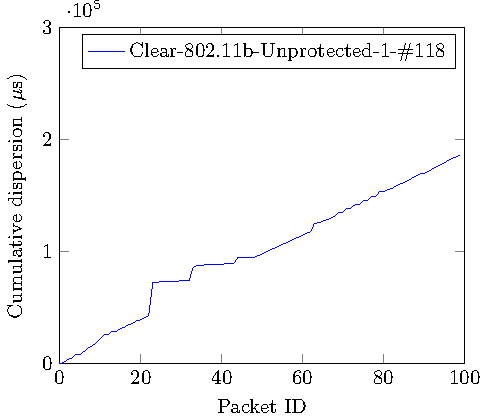
\includegraphics[width=\columnwidth]{plot-measurements-delta-delta}
  \end{minipage}
  \hfill
  \begin{minipage}{0.65\columnwidth}
  \begin{block}{Data efficiency}
    Given a train, try to split it into separate zones, remove coalescence and
    extract as much information as possible
  \end{block}
  \end{minipage}
  \end{minipage}
}


\subsection{The core procedure}

\frame{\frametitle{The core procedure}
  \begin{center}
  \tiny
  \begin{tikzpicture}[fill=LightBlue, node distance=0.1em]
    \newcommand*\pcount{6} \newcommand*\lastx{1}
    \begin{scope}[start chain=1 going left, minimum width=4em]
      \node [draw, fill, on chain=1] (t1) {Probe 1};
      \foreach \x [remember=\x as \lastx] in {2,...,\pcount} {
        \node [draw, fill, on chain=1] (t\x) {Probe \x};
        \draw [|-|] ($(t\x.north west)+(0,1em)$) -- ($(t\lastx.north west)+(0,1em)$);
      }
      \draw [|-|] ($(t\lastx.south west)+(0,-1em)$) --
        node[below] {ADR} ($(t1.south west)+(0,-1em)$);
      \node [draw, fill, on chain=1, left=1.8em of t\lastx, opacity=0.2,
        path fading=west] (t\lastx) {Probe 1};
    \end{scope}
    \draw[-stealth, dashed, black] ($(t1.east)+(0.5em,0)$) -- ++(3em,0);
    \coordinate (pipetopleft) at ($(t\pcount.north west)+(-1.5em,0.2em)$);
    \coordinate (pipetopright) at ($(t1.north east)+(0.5em,0.2em)$);
    \coordinate (pipebottomleft) at ($(t\pcount.south west)+(-1.5em,-0.2em)$);
    \coordinate (pipebottomright) at ($(t1.south east)+(0.5em,-0.2em)$);
    \draw (pipetopleft) -- (pipetopright) -- ++(3.5em,0);
    \draw (pipebottomleft) -- (pipebottomright) -- ++(3.5em,0);
  \end{tikzpicture}
  \end{center}

  \begin{center}
  \begin{minipage}{0.95\columnwidth}
  \begin{minipage}{0.6\columnwidth}
  \begin{block}{~}
  \begin{itemize}
  \item Send maximum-size packets
  \item Start with trains of 40 packets
  \item Gradually increase train length
  \end{itemize}
  \end{block}
  \vspace{1em}
  \pause
  \end{minipage}
  \hfill
  \begin{minipage}{0.3\textwidth}
  \newcommand*\jumpstatsfile{Clear-802.11g-WPA2-2}
  \includegraphics[width=\columnwidth, page=5]{\jumpstatsfile}
  \end{minipage}
  \end{minipage}
  \end{center}
}

\frame{\frametitle{The core procedure (cont.)}
  \begin{columns}
  \begin{column}{0.6\columnwidth}
  \begin{block}{~}
  \begin{itemize}
  \item Proceed round by round
  \begin{itemize}\item Why rounds?\end{itemize}
  \end{itemize}
  \end{block}
  \end{column}
  \begin{column}{0.3\textwidth}
  \end{column}
  \end{columns}
  \pause

  \vspace{-3\baselineskip}
  \begin{flushleft}
  \footnotesize
  \newcommand\fntsz{\Large}
  \visible<+->{\resizebox{0.32\columnwidth}{!}{\begin{tikzpicture}
  \newcommand*\tcount{6} \newcommand*\pcount{4}
  \begin{scope}[start chain=1 going below, minimum width=2em]
  \foreach \train [remember=\train as \lastt] in {1,...,\tcount} {
    \edef\tempa{\train} \edef\tempb{\the\numexpr\tcount-1\relax}
    \ifx\tempa\tempb
      \node [on chain=1] {};
      \foreach \x in {1,...,\pcount} {
        \node [below of=t-\lastt-\x] {$\vdots$};
      }
    \else
      \begin{scope}[fill=LightBlue, node distance=1em, minimum width=4em]
        \newcommand*\lastx{1}
        \node [draw, fill, on chain=1] (t-\train-1) {Probe 1};
        \begin{scope}[start branch=left, node distance=0.1em]
          \foreach \x [remember=\x as \lastx] in {2,...,\pcount} {
            \node [draw, fill, on chain=going left] (t-\train-\x) {Probe \x};
          }
        \end{scope}
        \draw ($(t-\train-\pcount.north west)+(-1em,0.2em)$) --
          ($(t-\train-1.north east)+(1em,0.2em)$);
        \draw ($(t-\train-\pcount.south west)+(-1em,-0.2em)$) --
          ($(t-\train-1.south east)+(1em,-0.2em)$);
      \end{scope}
    \fi
  }
  \end{scope}
  \coordinate (first-first) at ($(t-1-1.north east)+(1.5em,0.2em)$);
  \coordinate (first-last) at ($(t-1-\pcount.north west)+(-1.5em,0.2em)$);
  \coordinate (last-first) at ($(t-\tcount-1.south east)+(1.5em,-0.2em)$);
  \draw[decorate, decoration={brace,amplitude=0.5em}, black!90]
    (first-first) -- (last-first)
    node[midway,anchor=west,xshift=1.5em, rotate=-90, anchor=south] {\fntsz $T$ trains};
  \node [draw, fill=LightBlue!30, minimum width=\pcount*4.1em, minimum height=5ex]
    at ($(t-\tcount-1.south west)!0.5!(t-\tcount-\pcount.south east)-(0,2em)$)
    (computations) {Computations};
  \draw[decorate, decoration={brace,amplitude=0.5em}, black!90]
    (first-last |- computations.south east) -- (first-last)
    node[midway,anchor=east,xshift=-1.5em, rotate=90, anchor=south]
    {\fntsz Whole execution};
  \xcancelthistikz<+->[very thick, red]
  \end{tikzpicture}}}
  \;
  \visible<.->{\resizebox{0.28\columnwidth}{!}{\begin{tikzpicture}
  \begin{scope}[start chain=1 going below, minimum width=2em]
  \newcommand*\tcount{4} \newcommand*\pcount{4}
  \foreach \train [remember=\train as \lastt] in {1,...,\tcount} {
    \edef\tempa{\train} \edef\tempb{\the\numexpr\tcount-1\relax}
    \ifx\tempa\tempb
      \node [on chain=1] {};
      \foreach \x in {1,...,\pcount} {
        \node [below=3.3em of t-\lastt-\x] {$\vdots$};
      }
    \else
      \begin{scope}[fill=LightBlue, node distance=1.5em, minimum width=4em]
        \newcommand*\lastx{1}
        \node [draw, fill, on chain=1] (t-\train-1) {Probe 1};
        \begin{scope}[start branch=left, node distance=0.1em]
          \foreach \x [remember=\x as \lastx] in {2,...,\pcount} {
            \node [draw, fill, on chain=going left] (t-\train-\x) {Probe \x};
          }
        \end{scope}
        \draw ($(t-\train-\pcount.north west)+(-1em,0.2em)$) --
          ($(t-\train-1.north east)+(1em,0.2em)$);
        \draw ($(t-\train-\pcount.south west)+(-1em,-0.2em)$) --
          ($(t-\train-1.south east)+(1em,-0.2em)$);
        \node [on chain=1] {};
        \node [draw, fill=LightBlue!30, minimum width=\pcount*4.1em, minimum height=4ex]
          at ($(t-\train-1.south west)!0.5!(t-\train-\pcount.south east)-(0,1.5em)$)
          (c-\train) {Computations};
      \end{scope}
    \fi
  }
  \coordinate (first-first) at ($(t-1-1.north east)+(1.5em,0.2em)$);
  \coordinate (first-last) at ($(t-1-\pcount.north west)+(-1.5em,0.2em)$);
  \coordinate (last-first) at ($(t-\tcount-1.south east)+(1.5em,-0.2em)$);
  \draw[decorate, decoration={brace,amplitude=0.5em}, black!90]
    (first-last |- c-\tcount.south east) -- (first-last)
    node[midway,anchor=east,xshift=-1.5em, rotate=90, anchor=south]
    {\fntsz Whole execution};
  \end{scope}
  \xcancelthistikz<+->[very thick, red]
  \end{tikzpicture}}}
  \;
  \visible<.->{\resizebox{0.32\columnwidth}{!}{\begin{tikzpicture}
  \newcommand*\tcount{4} \newcommand*\pcount{4}
  \begin{scope}[start chain=1 going below, minimum width=2em]
  \foreach \x in {1,2} {
    \foreach \train [remember=\train as \lastt] in {1,...,\tcount} {
      \edef\tempa{\train} \edef\tempb{\the\numexpr\tcount-1\relax}
      \ifx\tempa\tempb
        \node [on chain=1] {};
        \foreach \x in {1,...,\pcount} {
          \node [below of=t-\lastt-\x] {$\vdots$};
        }
      \else
        \begin{scope}[fill=LightBlue, node distance=1em, minimum width=4em]
          \newcommand*\lastx{1}
          \node [draw, fill, on chain=1] (t-\train-1) {Probe 1};
          \begin{scope}[start branch=left, node distance=0.1em]
            \foreach \x [remember=\x as \lastx] in {2,...,\pcount} {
              \node [draw, fill, on chain=going left] (t-\train-\x) {Probe \x};
            }
          \end{scope}
          \draw ($(t-\train-\pcount.north west)+(-1em,0.2em)$) --
            ($(t-\train-1.north east)+(1em,0.2em)$);
          \draw ($(t-\train-\pcount.south west)+(-1em,-0.2em)$) --
            ($(t-\train-1.south east)+(1em,-0.2em)$);
        \end{scope}
      \fi
    }
    \node [on chain=1] {};
    \node [draw, fill=LightBlue!30, minimum width=\pcount*4.1em, minimum height=5ex]
      at ($(t-\tcount-1.south west)!0.5!(t-\tcount-\pcount.south east)-(0,2em)$)
      (computations) {Computations};
    \coordinate (first-first) at ($(t-1-1.north east)+(1.5em,0.2em)$);
    \coordinate (first-last) at ($(t-1-\pcount.north west)+(-1.5em,0.2em)$);
    \coordinate (last-first) at ($(t-\tcount-1.south east)+(1.5em,-0.2em)$);
    \draw[decorate, decoration={brace,amplitude=0.5em}, black!90]
      (first-first) -- (last-first)
      node[midway,anchor=west,xshift=1.5em, rotate=-90, anchor=south]
      {\fntsz $M$ trains};
    \draw[decorate, decoration={brace,amplitude=0.5em}, black!90]
      (first-last |- computations.south east) -- (first-last)
      node[midway,anchor=east,xshift=-1.5em, rotate=90, anchor=south] {\fntsz Round};
    \def\tempa{1}
    \ifx\x\tempa
      \node [on chain=1] {};
      \foreach \x in {1,...,\pcount} {
        \node [below=4em of t-\tcount-\x] {$\vdots$};
      }
    \fi
  }
  \end{scope}
  \end{tikzpicture}}}
  \end{flushleft}
}

\frame{\frametitle{The core procedure (cont.)}
  \tiny
  \begin{tikzpicture}[fill=LightBlue, node distance=0.1em]
    \newcommand*\pcount{6} \newcommand*\lastx{1}
    \begin{scope}[start chain=1 going left, minimum width=4em]
      \node [draw, fill, on chain=1] (t1) {Probe 1};
      \foreach \x [remember=\x as \lastx] in {2,...,\pcount} {
        \node [draw, fill, on chain=1] (t\x) {Probe \x};
        \draw [|-|] ($(t\x.north west)+(0,1em)$) -- ($(t\lastx.north west)+(0,1em)$);
      }
      \draw [|-|] ($(t\lastx.south west)+(0,-1em)$) -- ($(t1.south west)+(0,-1em)$);
    \end{scope}
    \draw[-stealth, dashed, black] ($(t1.east)+(0.5em,0)$) -- ++(1em,0);

    \draw[decorate, decoration={brace,amplitude=0.5em}, black!90]
      ($(t\pcount.north west)+(0,2em)$) -- ($(t2.north east)+(0,2em)$);
    \draw[decorate, decoration={brace,amplitude=0.5em}, black!90]
      ($(t2.south east)+(0,-2em)$) -- ($(t\pcount.south west)+(0,-2em)$);

    \coordinate (pointa) at ($(t\pcount.north west)!0.5!(t2.north east)+(0,2em)$);
    \coordinate (pointb) at ($(t\pcount.south west)!0.5!(t2.south east)-(0,2em)$);
    \draw [->] ($(pointa)+(0,0.5em)$) -- ++(0,1em);
    \draw [->] ($(pointb)-(0,0.5em)$) -- ++(0,-1em);
    \alt<1>{
      \node [anchor=south east] at ($(t1.north west)+(1em,3.5em)$)
        {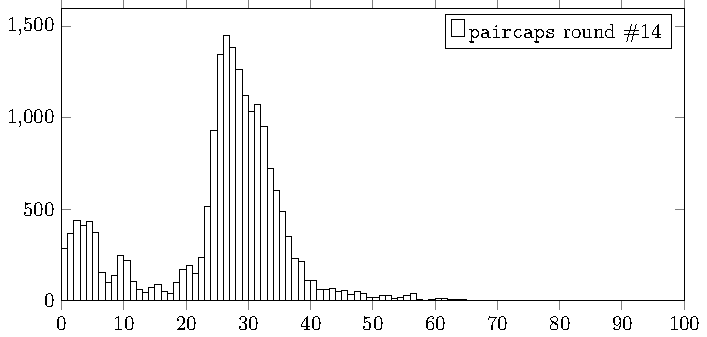
\includegraphics[width=23em,page=1]{plot-execution}};
      \node [anchor=north east] at ($(t1.south west)+(1em,-3.5em)$)
        {\includegraphics[width=22em,page=3]{plot-execution}};
    }{
      \node [anchor=south east] at ($(t1.north west)+(1em,3.5em)$)
        {\includegraphics[width=23em,page=2]{plot-execution}};
      \node [anchor=north east] at ($(t1.south west)+(1em,-3.5em)$)
        {\includegraphics[width=22em,page=4]{plot-execution}};
    }

    \node[anchor=west, yshift=2em] at ($(t1.east)+(2em,0)$) {%
      \begin{minipage}{20em}\footnotesize
      \begin{block}{Calculations at each round}
      \begin{itemize}
      \item Calculate pair capacities % from successive packets in each train
      % (filter and remove dispersions affected by IC)
      \item Calculate ADR capacities % for each train
      % (ignore if pseudo-IC affects the beginning or the end of the train)
      \item Calculate distribution
      \item Calculate bin width
      \item<2-> Extract modes % of all gathered path and ADR capacities
      \item<2-> Estimate (temporary) capacity
      \end{itemize}
      \end{block}
      \end{minipage}
    };
  \end{tikzpicture}
}


\subsection{Pseudo-IC}

\frame{\frametitle{Detect pseudo-IC}
  \begin{block}{Filtering capacities from IC}
  Detecting interrupt coalescence is a critical task
  \end{block}
  \pause

  \begin{exampleblock}{Idea}
  Why do not reduce the receiver's buffer size by means of \texttt{setsockopt},
  to reduce or completely suppress IC?
  \end{exampleblock}
  \pause

  \begin{alertblock}{Wrong}
  Option \texttt{SO\_RCVBUF} affects only a buffer related to the \emph{UDP
  socket}, and has nothing to do with the kernel's buffer used by NIC.

  In fact, the receiver's buffer should be as large as possible, to reduce
  (late) packet drops.
  \end{alertblock}
}

\FrameRIMOSSO{
  \begin{center}\footnotesize
  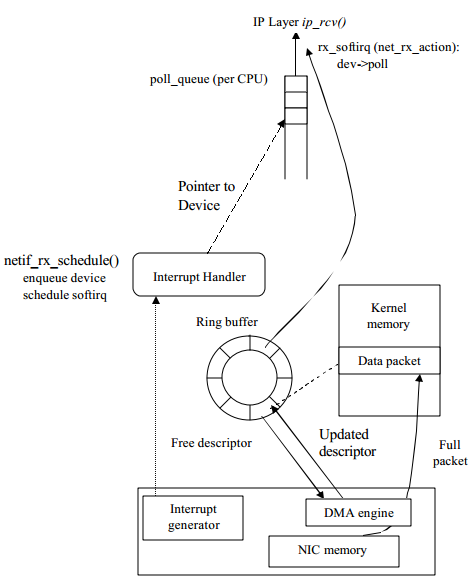
\includegraphics[width=0.5\textwidth]{napi-datatag}
  \begin{tikzpicture}[fill=LightBlue, text width=\widthof{Generator}]
  % NIC hardware
  \node [draw, align=center]
    (dma) {DMA Engine};
  \node [draw, below=of dma, align=center]
    (int-gen) {Interrupt Generator};
  \draw [blue, dashed] ($(dma.north east)+(1em,3em)$) -- ($(int-gen.south east)+(1em,-3em)$)
    node[left] {NIC Hardware};
  % Device driver
  \node [draw, circle, right=of dma, text width=2em, align=center]
    (dmaring-inner) {DMA Ring};
  \node [draw, circle, minimum size=5.5em] (dmaring-outer) at (dmaring-inner) {};
  \foreach \a in {0, 30, ..., 330}
    \draw (dmaring-inner.\a) -- (dmaring-outer.\a);
  \node [draw, align=center]
    (int-handler) at (dmaring-outer |- int-gen) {Interrupt Handler};
  \draw [blue, dashed] ($(dmaring-outer.north east)+(1.4em,2.5em)$) --
    ($(int-handler.south east)+(1em,-3em)$) node[left, align=center] {Device driver};

  \draw[-stealth, black] (dma) -- ($(dmaring-outer.105)!0.5!(dmaring-inner.105)$);
    node[left] {\tiny{update descriptor}};
  \draw[-stealth, black, dotted] (int-gen) -- (int-handler);
  % Kernel space
  \begin{scope}[start chain=1 going right, node distance=0.1em,
      minimum width=0.8em, minimum height=2.5em, text width=0]
    \node [draw, fill, on chain=1, right=3em of dmaring-outer] (tail) {};
    \node [draw, fill, on chain=1] {};
    \node [draw, fill, on chain=1] {};
    \node [draw, fill, on chain=1] (head) {};
  \end{scope}
  \draw[black, thick, dotted, -stealth] (head.east) -- ++(2em,0) node[right]{IP layer};
%  \draw ($(tail.north west)+(-0.5em,0.2em)$) -- ($(head.north east)+(0.5em,0.2em)$);
%  \draw ($(tail.south west)+(-0.5em,-0.2em)$) -- node[below] {Buffer}
%    ($(head.south east)+(0.5em,-0.2em)$);
  % User space
  \node [draw, fill, right=3em of head] (app) {Application};

  \draw[-stealth, black] ($(dmaring-outer.105)!0.5!(dmaring-inner.105)$) -- (tail);
  \end{tikzpicture}
  \end{center}
}

\frame{\frametitle{Detect pseudo-IC (cont.)}
  \begin{columns}[c]
  \begin{column}{0.5\columnwidth}
  \includegraphics[width=\columnwidth, page=2]{plot-measurements-delta-delta}
  \end{column}
  \begin{column}{0.5\columnwidth}
  \alt<2>{
    \includegraphics[width=\columnwidth, page=4]{plot-measurements-delta-delta}
  }{
    \includegraphics[width=\columnwidth, page=3]{plot-measurements-delta-delta}
  }
  \pause
  \begin{alertblock}{~}<2>\centering $\displaystyle
    \frac{1500\times8~\text{bit}}{183\unit{\mu s}} \approx 65.6\unit{Mbps} $
  \end{alertblock}
  \end{column}
  \end{columns}
}

\frame{\frametitle{Detect pseudo-IC (cont.)}
  \begin{minipage}{\columnwidth}
  \begin{minipage}{0.47\columnwidth}
  \includegraphics[width=\columnwidth, page=4]{plot-measurements-delta-delta}
  \end{minipage}
  \hfill
  \begin{minipage}{0.47\columnwidth}
  \alt<2>{
    \includegraphics[width=\columnwidth, page=8]{plot-measurements-delta-delta}
  }{
    \includegraphics[width=\columnwidth, page=7]{plot-measurements-delta-delta}
  }
  \pause
  \end{minipage}
  \end{minipage}
}

\frame{\frametitle{Detect pseudo-IC (cont.)}
  \begin{minipage}{\columnwidth}
  \begin{minipage}{0.47\columnwidth}
  \alt<2->{
    \includegraphics[width=\columnwidth, page=6]{plot-measurements-delta-delta}
  }{
    \includegraphics[width=\columnwidth, page=5]{plot-measurements-delta-delta}
  }
  \end{minipage}
  \hfill
  \begin{minipage}{0.47\columnwidth}
  \visible<3>{
    \includegraphics[width=\columnwidth, page=9]{plot-measurements-delta-delta}
  }
  \end{minipage}
  \end{minipage}

  \begin{exampleblock}{Two \emph{features}}
    \begin{center}\small\rulecolor{OliveGreen!90}
    \begin{tabular}{l>{$\Rightarrow$}cl}
    Packet pair dispersion           & & Minimum possible dispersion \\
    \pause
    Packet pair dispersion           & & Kernel-to-user latency      \\
    \pause
    Delta of packet pair dispersions & & Kernel-to-user latency
    \end{tabular}
    \end{center}
  \end{exampleblock}
}

\frame{\frametitle{Final capacity estimate}
  \begin{minipage}{\columnwidth}
  \begin{minipage}{0.59\columnwidth}
  Procedure:
  \begin{itemize}
  \item Proceed round by round
  \item Do calculations at the end of each round
  \item Try to determine the path capacity
  \item Check for convergence of partial results
  \end{itemize}
  \end{minipage}
  \hfill
  \begin{minipage}{0.39\columnwidth}
  \includegraphics[width=\columnwidth, page=5]{plot-execution}
  \end{minipage}
  \end{minipage}

  \bigskip
  Typical results:
  \begin{itemize}
  \item Execution time: \hfill \textcolor{red}{$15\div30$ mins}
        \visible<2>{$\quad\Rightarrow\quad$ \textcolor{green}{$1\div 2$ mins}}
        \hfill\null
  \item Generated traffic: \hfill \textcolor{red}{$100\div180$\,MB}
        \visible<2>{$\quad\Rightarrow\quad$ \textcolor{green}{$15\div30$\,MB}}
        \hfill\null
  \end{itemize}
}


\frame{\frametitle{Questions?}
  \begin{minipage}{\columnwidth}
  \begin{minipage}{0.4\columnwidth}
  \begin{center}
  \color{blue}\Huge
  Questions
  \end{center}
  \end{minipage}
  \begin{minipage}{0.55\columnwidth}
  
\includegraphics[width=15em]{questionmark}
  \end{minipage}
  \end{minipage}
}


\frame[allowframebreaks]{\frametitle{\refname}
  \renewcommand*{\bibfont}{\scriptsize}
  \nocite{*}
  \printbibliography[heading=references]
}

\end{document}
